\documentclass{article}


\usepackage{arxiv}

\usepackage[utf8]{inputenc} % allow utf-8 input
\usepackage[T1]{fontenc} % use 8-bit T1 fonts
\usepackage{hyperref} % hyperlinks
\usepackage{url} % simple URL typesetting
\usepackage{booktabs} % professional-quality tables
\usepackage{amsmath}
\usepackage{amssymb}
\usepackage{mathtools}
\usepackage{amsfonts} % blackboard math symbols
\usepackage{nicefrac} % compact symbols for 1/2, etc.
\usepackage{microtype} % microtypography
\usepackage{lipsum}
\usepackage{graphicx}
\graphicspath{ {./images/} }
\title{Extending Neural Collaborative Filtering}

\author{
Shriram Varadarajan \\
Department of Electrical and Computer engineering\\
University of Iowa\\
Iowa City, IA, 52242 \\
\texttt{shriram-varadarajan@uiowa.edu} \\
%% examples of more authors
\And
Jacob Nishimura \\
Department of Electrical and Computer engineering\\
University of Iowa\\
Iowa City, IA, 52242 \\
\texttt{jacob-nishimura@uiowa.edu} \\
\And
Joseph Kim \\
Department of Biomedical Engineering\\
University of Iowa\\
Iowa City, IA, 52242 \\
\texttt{joseph-kim-3@uiowa.edu} \\
%% \AND
%% Coauthor \\
%% Affiliation \\
%% Address \\
%% \texttt{email} \\
%% \And
%% Coauthor \\
%% Affiliation \\
%% Address \\
%% \texttt{email} \\
%% \And
%% Coauthor \\
%% Affiliation \\
%% Address \\
%% \texttt{email} \\
}


\begin{document}
\maketitle

\begin{abstract}
This is our paper for the course ISE:6380 Deep learning course taught by Prof. Stephen Baek, University of Iowa. This will be modified and updated through the course of the semester.
\end{abstract}


% keywords can be removed
\keywords{Collaborative filtering \and Recommender systems \and Content-based filtering}


\section{Introduction}
In the current age of web browsing, recommendations are given in numerous applications ranging from entertainment to shopping to social media. Many systems have far too many items for a user to consistently find compelling content on their own. For example, the iOS app store has millions of apps, Amazon's marketplace has hundreds of millions of items, and YouTube hosts billions of videos. Recommendations are user-personalized suggestions derived from known interests from past experiences or behavior. Recommendation (or recommender) systems are systems which use various algorithms to generate and rank suggestions to show the user. While users can find items using search, recommender systems are able to surface items the user may not have thought of or even knew existed. Good recommender systems can yield benefits for both the user and the business: users can be given more relevant and compelling recommendations leading to a better experience, and a better experience can promote more user engagement and growth.

In general, recommender systems are composed of three parts: candidate generation, scoring, and re-ranking. The recommender system takes in a single or numerous queries (information about the user such as an ID number or previous interactions, and other context such as the time of day or the user's device) and outputs a set of items (such as movies, apps, social media posts). The candidate generation stage (which may consist of multiple, separate generators) uses the queries to select a small (relative to the total amount of items in the system) set of items for further processing. The scoring stage takes in the generated candidates, determines a score for each item, and ranks the items according to that score. Finally, the re-ranking stage can consider additional criteria to change the recommendations before being served to the user. Items can be moved or discarded in this stage for business reasons (removing content the user isn't eligible to play, filtering out mature content) or for recommendation quality reasons (freshness, diversity, etc).

Focusing on candidate generation, multiple approaches are used today. Two common approaches are content-based filtering or collaborative filtering. Both approaches utilize embeddings (projections from high-dimensional, categorical information to relatively low-dimensional, continuous vector representations) to determine similarity between entities. Content-based filtering finds similar items to those the user has already indicated they like. For example, if a user has shown that they enjoy action novels, the system can find similar action novels to recommend the user. Some advantages to content-based filtering are it does not need other user’s information to make recommendations, and it can capture the specific interests of the user. A large downside to content-based filtering is it can require a lot of domain knowledge to extract relevant features. Content-based filtering typically uses explicit feedback, such as numeric ratings the user gives to novels they've read.

Unlike content-based filtering, collaborative filtering uses interest data from other users to power its recommendations. Collaborative filtering is built off the assumptions that users with similar interactions share some number of preferences, and users that have shared preferences may respond similarly to the same items. For example, given users A and B have both bought some of the same items in the past, a new item that user A buys may also interest user B. Collaborative filtering has the advantage of not requiring large amounts of domain knowledge, as the system is able to learn effective embeddings for the data by itself. It is also able to recommend the user new items that are separate from the user's current known interests (serendipity). A major downside to collaborative filtering is that collaborative filtering cannot handle new items that the system has come up with since it is difficult to create embeddings for items that the model hasn’t seen yet. Unlike content-based filtering, collaborative filtering can often also use implicit feedback, such as assuming the user is interested in each item they've bought. While this can have drawbacks, such as aiding "clickbait" content, it also generally allows much greater amounts of data to be used for learning.

Traditionally, collaborative filtering uses Matrix Factorization (MF) to learn and utilize an embedding model. Using user-item interactions as inputs to a Matrix Factorization model allows the model to learn embeddings for the users and items. The model can then be used for new user-item pairs by calculating the dot product between the user's embedding and the item's embedding: $\hat{y}_{ui} = f(u,i|p_u,q_i) = \textbf{p}^T_u\textbf{q}_i = \sum{p_{uk}q_{ik}}$, where $\hat{y}_{ui}$ is the interaction and $\textbf{p}_u$ and $\textbf{q}_i$ are the embedding vectors for user \textit{u} and item \textit{i}.

He et al. proposed Neural Collaborative Filtering (NCF) as a new framework for collaborative filtering which combines traditional MF with a multilayer perceptron to better recommendation performance compared to previous MF-based techniques (element-wise Alternating Least Squares, Bayesian Personalized Ranking)[1]. The original NCF paper uses a multilayer perceptron to model additional non-linearities in user-item interactions. Further, He et al. proposed Outer Product-based Neural Collaborative filtering, a technique which applied the outer product operation to user and item embeddings generating a 2-dimensional interaction map[2]. The approach can then use Convolutional Neural Network models on the interaction map to extract features and finally predict the interaction. In both cases, the frameworks encourage further experimentation with network architecture and parameters to imrpove performance.

In this manuscript, the authors propose applying recent advances in neural network training (batch normalization, dropout) and architecture to the inner and outer product NCF frameworks.

%\subsection{Related works}
%Neural collaborative filtering - \url{https://arxiv.org/pdf/1708.05031.pdf}. \\
%Visually explainable recommendation - \url{https://arxiv.org/pdf/1801.10288.pdf}. \\
%Makeup recommendations = %\url{https://www.researchgate.net/publication/309919310_Examples-Rules_Guided_Deep_Neural_Network_for_Makeup_Recommendation}. \\
%Outer product NCF - \url{https://arxiv.org/pdf/1808.03912.pdf}.

\section{Problem Definition}
\label{sec:Problem Definition}
To test the effectiveness of our modifications to the NCF and outer-product frameworks, they will be applied to the problem of generating movie recommendations based on implicit feedback. Given $M$ users, $N$ items, and an $M$x$N$ user-item matrix, $\bold{Y}$, $y_{ui} = 1$ if user $u$ has interacted with item $i$, otherwise $y_{ui} = 0$. He et al. points out this can pose challenges as a value of 1 doesn't necessarily mean the user liked an item, and a value of 0 doesn't mean the user dislikes the item (they may just be unaware of that item)[1]. The recommendation problem is then given as the problem of estimating scores for unobserved user-item pairs in $\bold{Y}$.

The deep neural networks to be compared will be built using TensorFlow with Keras and will take in a pair consisting of user ID and movie ID. The networks will then output a probability that the user would interact with the movie. To evaluate the performance of the models, the authors will use 2 metrics: Hit Ratio (HR) and Normalized Discounted Cumulative Gain (NDCG). To calculate these metrics, the models will be fed in 99 items that the user hasn't interacted with and 1 test item that the user has interacted with. Hit Ratio measures whether the test item appears in the top-N of the 100 ranked items. Normalized Discounted Cumulative Gain measures how-highly the item is ranked within the top-N.

The traditional Neural Collaborative Filtering model will take the user and item embeddings, apply Matrix Factorization and a neural network to the embeddings, and have a final block of layers to compute the probability. The outer-product Neural Collaborative Filtering model will also take the user and item embeddings. This model will compute the outer product between the two embeddings, resulting in a 2-dimensional, $d$x$d$ matrix known as the interaction map. CNN architectures such as VGG, ResNet, or DenseNet can be applied to the interaction map to extract features, and a final block of layers can again compute the probability.

\textbf{Inputs}: The input to our models will be pairs of user ID and movie ID converted into Dense vectors using embeddings. Each Dense embedded vector will have $d$ dimensions, where d is an adjustable parameter for the size of the embedding.

\textbf{Outputs}: The output of our models is a probability between 0 and 1. The probability represents the likelihood that a user $u$ would interact with an item $i$.

\section{Data}
\label{sec:Data}

\begin{itemize}
\item Available data include user-given movie ratings, user-applied movie tags, and two additional files containing links to each movie's IMDB and TMDB. The movie ratings contain unique identifiers for the user and the movie, a rating score, and the time the rating was made. The movies also have associated genres and titles. Data that is not available include users' text reviews for further word processing and text similarity.
\item The movies were collected from the website \url{https://www.themoviedb.org/} by the GroupLens research group at the University of Minnesota Twin Cities. This database hosts information on millions of movies, TV shows, and actors. The site was originally conceived as a donation from the Online Media Database, which is an online collaborative database intended to share content published under a Creative Commons license. The data was created by 162,541 users between January 09, 1995 and November 21, 2019. This dataset was generated on November 21, 2019.
\item MovieLens datasets are generally distributed in the CSV format. The authors use the built-in CSV parser in the pandas library to extract the data. GroupLens distributes a multitude of datasets for various uses (education, research, performance testing). The authors propose using the latest small dataset for initial development and training, then switching to the stable 1M dataset for performance comparisons. The small dataset is formatted with 100,836 ratings, 3683 tags, 9,742 movies, and 610 users collected between March 1996 and September 2018. The stable 1M dataset has 1 million ratings from 6000 users on 4000 movies.

\end{itemize}

%\subsection{Figures}
%Figures \\
%See Figure \ref{fig:fig1}. Here is how you add footnotes. \footnote{Sample of the first footnote.}


%\begin{figure}
%\centering
%\fbox{\rule[-.5cm]{4cm}{4cm} \rule[-.5cm]{4cm}{0cm}}
%\caption{Sample figure caption.}
%\label{fig:fig1}
%\end{figure}

\subsection{Tables}

%Table~\ref{tab:table1}.

\begin{table}[h]
\caption{Ratings}
\centering
\begin{tabular}{llll}
\toprule
userId & movieId & Rating & Timestamp \\
\midrule
1 & 1 & 4 & 964982703 \\
1 & 3 & 4 & 964981247 \\
1 & 6 & 4 & 964982224 \\
\bottomrule
\end{tabular}
\label{tab:table1}
\end{table}

\begin{table} [h]
\caption{Tags}
\centering
\begin{tabular}{llll}
\toprule
userId & movieId & Tag & Timestamp \\
\midrule
2 & 60756 & funny & 1445714994 \\
2 & 60756 & Highly quotable & 1445714996 \\
2 & 60756 & will ferrell & 1445714992 \\
\bottomrule
\end{tabular}
\label{tab:table2}
\end{table}

\begin{table}[h]
\caption{MovieLens}
\centering
\begin{tabular}{llll}
\toprule
Users & Movies & Ratings \\
\midrule
6040 & 3076 & 1000203 \\
\bottomrule
\end{tabular}
\label{tab:table1}
\end{table}

\section{Experiments and Results}
\subsection{Evaluation charts and results}
\subsubsection{Hit Rate and NCDG @ K=10}
In this section, we tabulate and present the results of training our various models on the MovieLens dataset. \\
HitRate@10 and NCDG@10 (Normalized cumulative distributed gain) for the models are presented below. These evaluations were calculated using the top-N recommendations that were predicted by the models. The models are tested over 11 epochs with the 0th epoch being the initial testing of the model.\\
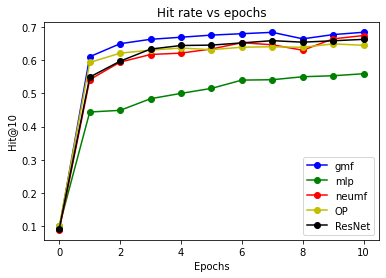
\includegraphics[scale=0.5]{hit_rate}
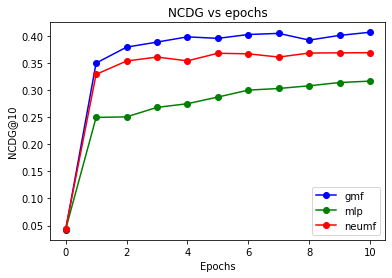
\includegraphics[scale=0.5]{ncdg}\\

\subsubsection{Loss}
Loss for the models is presented in the chart below. Loss was calculated as the binary cross-entropy from the keras library. The accuracy and the loss metrics for all the models was calculated using binary crossentropy since the ratings were implicit, using binary values of 0 and 1. \\
\begin{center}
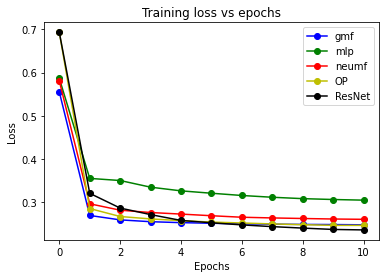
\includegraphics[scale=0.5]{loss}
\end{center}

\subsubsection{GMF on the 100k dataset}
 The models were first trained on the 100k Movielens dataset but the errors and the evaluation metrics were far too off to predict any recommendations for the users. Specifically, the 100k dataset with 100,000 ratings was trained on the GMF model and the results of the evaluations and the loss is depicted in the chart below.
The model was tested on the Hit rate, NCDG and binary loss over 11 epochs with the 0th epoch being the initial testing of the model. \\
\begin{center}
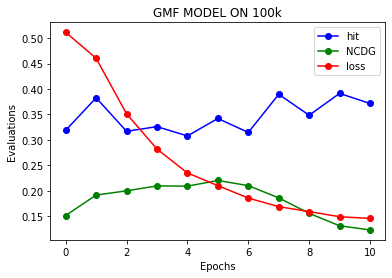
\includegraphics[scale=0.5]{gmf100k}
\end{center}

\subsubsection{Embedding dimensions on model performance}
We tested the models' loss and metrics against embedding vector dimensions of sizes 4, 8, 16 and 32 since they are common powers of 2. As can be observed from the figure, GMF and NeuMF models performed really well on 16 dimensions os the inputs whereas the MLP model did well on the dimension of 4. this could be due to the fact that the MLP model has a lot of parameters than the GMF model and thus might result in overfitting the training dataset. As far as NeuMF is concerned, even though the number of parameters were more or less the same, as will be descirbed in the Combined NeuMF section, the $\alpha$ parameter reduces its effect on the overall output.
\begin{center}
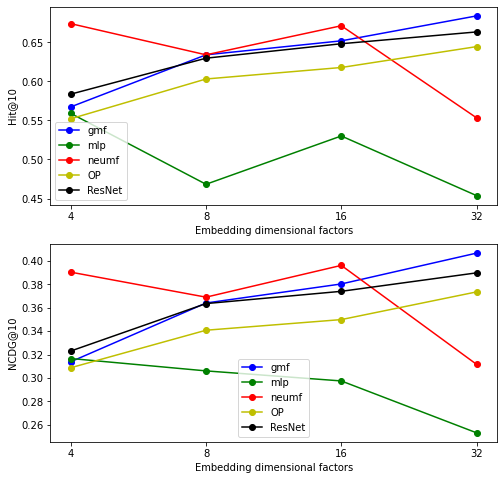
\includegraphics[scale=0.5]{factors}
\end{center}

\subsection{Multi-layer Preceptron}
The multi-layer preceptron model used a 64 $\rightarrow$ 32 $\rightarrow$ 16 $\rightarrow$ 1 dense layer units with a RelU activation for the first 3 layers and the sigmoid activation for the last Dense 1 unit layer. The first layer is initialized using a glorot uniform initializer and uses an L2 regularizer. The other layers use a normal configuration. This model was previously tested with an average ayer configuration such as 512 $\rightarrow$ 256 $\rightarrow$ 64 $\rightarrow$ 32 and 32 $\rightarrow$ Avg layer $\rightarrow$ 1 that used more dense units and layers with an addition of an average layer that smooths the result of the 32 units dense layers. But the model had a problem of overfitting the dataset. The metrics of the tested models are presented in the table below.

\begin{table}[h]
\caption{Accuracies, HR@10 and NCDG@10}
\centering
\begin{tabular}{llll}
\toprule
Model & Accuracy & HR10 & NCDG10 \\
\midrule
Original Model & 0.863 & 0.5629 & 0.3145 \\
Average model & 0.814 & 0.4412 & 0.2216 \\
\bottomrule
\end{tabular}
\label{tab:table6}
\end{table}

\subsection{Generalized Matrix Factorization}
GMF model used the matrix factorization method of the dot product bwtween the user latent vector and the item latent vector.

\subsection{Combined NeuMF}
The NeuMF model combined the matrix factorization and the multi-layer preceptron. The GMF model is the same as the original wheras the MLP part had some tweaking to it. Instead of the original layers that were mentioned in Table 4, the model uses 64 $\rightarrow$ 32 $\rightarrow$ 8 $\rightarrow$ 1, with L2 regularization on all the layers. After the individual part outputs, the model use a custom layer that combines the output of the GMF and the MLP models together using $\alpha$ as a weighting parameter to balance the effects of the two model outputs.\\

\[
\begin{bmatrix}
    \alpha * (\phi_{GMF}) \\
    (1 - \alpha) * (\phi_{MLP})  
\end{bmatrix}
\]

The final result is an addition operation performed on the elements of the matrix and this gives the prediction $y_{ui}$ of user \emph{u} and item \emph{i}.

\subsection{Outer Product Model}
The Outer Product model NCF model took in user and item embeddings similarly to the other MF models. However, the Outer Product model additionally computed the outer product between the two to create a 2-dimensional interaction map. This was followed by a convolution layer with ReLU activation, pooling, another convolution layer with ReLU activation, and a final Dense layer with sigmoid activation. This was additionally tested with varying embedding vector dimensions of sizes 8, 16, and 32.

\subsection{Outer Product Model - ResNet}


\section{Comparison of Models}
From the last section, all of the models strongly perform well on the datasets. We can see that GMF and NeuMF dominate MLP in terms of accuracy and evaluation metrics. Specifically, when comparing the best performances of these models across their embedding dimension factors, GMF and NeuMF show consistent improvements over MLP in terms of HR@10 and NCDG@10. GMF, in particular seems to be performing a little better than NeuMF by margins of $\pm 0.02$. MLP is lower than NeuMF by about $0.1 \pm 0.02$. MLP can be improved by adding more dense layers or adding regularizers, here we test with only 3 hidden layers.\\

We also see that the GMF model performs poorly on the 100k dataset in terms of the evaluation metrics even though the binary loss goes down for every epoch. The highest HR@10 achieved was $0.4$ on this dataset and NCDG@10 was around $0.25$. Comparing this to the models trained on the 1m dataset shows the difference. This might be due to the arrangement or the input type feed to the neural net. of the 100k dataset of MovieLens compared to the 1M dataset where the former consisted of tensor slices whereas the 1m dataset used numpy arrays which proved to be much faster to train the models.\\

The Outer Product model was similarly evaluated, primarily using HR and NCDG. Increasing embedding vector dimension size from 8 up to 32 allowed for greater HR and NCDG along with incremental decreases in loss. Notably, a learning rate of 0.001 using the Adam optimizer yielded the best performance compared to higher values. In direct comparison between LR = 0.001 and LR = 0.005, the lower value demonstrated greater decrease in loss, perhaps indicating unnecessarily quick convergence in the higher LR model leading to a suboptimal outcome.\\

The Outer Product model was expanded to incorporate ResNet. Increased architectural complexity yielded similar results to the original model, with a comparison of $0.64$ HR and $0.37$ NCDG for the original versus \rule{1cm}{0.15mm} HR and \rule{1cm}{0.15mm} NCDG for the ResNet model after 20 epochs of training.\\

\bibliographystyle{unsrt}
%\bibliography{references} %%% Remove comment to use the external .bib file (using bibtex).
%%% and comment out the ``thebibliography'' section.


%%%% Comment out this section when you \bibliography{references} is enabled.
%\begin{thebibliography}{1}
%
%
%\bibitem{he2017}
%He, Xiangnan and Liao, Lizi and Zhang, Hanwang and Nie, Liqiang and Hu, 
% Xia and Chua, Tat-Seng
%\newblock Neural Collaborative Filtering.
%\newblock In {\em International World Wide Web Conferences Steering 
% Committee}. WWW, 2017.
%
%\bibitem{kour2014real}
%George Kour and Raid Saabne.
%\newblock Real-time segmentation of on-line handwritten arabic script.
%\newblock In {\em Frontiers in Handwriting Recognition (ICFHR), 2014 14th
% International Conference on}, pages 417--422. IEEE, 2014.
%
%\bibitem{kour2014fast}
%George Kour and Raid Saabne.
%\newblock Fast classification of handwritten on-line arabic characters.
%\newblock In {\em Soft Computing and Pattern Recognition (SoCPaR), 2014 6th
% International Conference of}, pages 312--318. IEEE, 2014.
%
%\bibitem{hadash2018estimate}
%Guy Hadash, Einat Kermany, Boaz Carmeli, Ofer Lavi, George Kour, and Alon
% Jacovi.
%\newblock Estimate and replace: A novel approach to integrating deep neural
% networks with existing applications.
%\newblock {\em arXiv preprint arXiv:1804.09028}, 2018.
%
%\end{thebibliography}


\end{document}